\documentclass[english]{beamer}
\usepackage[utf8]{inputenc}
\usepackage[T1]{fontenc}
\usepackage{amsfonts}
%\usepackage{amsthm}
\usepackage{makeidx}  % allows for indexgeneration
\usepackage{amsmath}
\usepackage{mathtools}
\usepackage{verbatim}
\usepackage{float}
\usepackage{graphicx}
\usepackage{times}  
%\usepackage[lined, boxed, linesnumbered]{algorithm2e}
\usepackage{array}
%\usepackage{makecell}
\usepackage{tikz}
\usetikzlibrary{positioning,arrows}
\usepackage{lscape}
\usepackage{caption}
\usepackage{subcaption}
%\usepackage{subfig}

\beamertemplatenavigationsymbolsempty
\setbeamertemplate{footline}[frame number]

\usetheme{Antibes} % Beamer theme v 3.0
\usecolortheme{beaver}

%\usebackgroundtemplate
%{
%  \includegraphics[width=\paperwidth,height=\paperheight]{columns.png}%
%}

\newtheorem{proposition}{Proposition}
%\newtheorem{corollary}{Corollary}
%\newtheorem{theorem}{Theorem}[section]
%\newtheorem{lemma}{Lemma}[section]

\title{Branch \& Price for the Virtual Network Embedding Problem}
\author{Leonardo F.S. Moura}
\date{March 2, 2015}
%\institute{Computer Science Department, Federal University of Rio Grande do Sul\\Porto Alegre, Brazil}
%\newtheorem{proposition}{Proposition}
%\newtheorem{theorem}{Theorem}[section]
%\newtheorem{lemma}{Lemma}[section]
\begin{document}
\begin{frame}
\titlepage

\begin{center}
\scriptsize
Advisor: Luciana S. Buriol
\begin{figure}
    \centering
    \includegraphics[scale=0.4]{inf.png}
\end{figure}
\end{center}
\end{frame}

%---------------------------
\begin{frame}
  \frametitle{Outline}
\begin{enumerate}
  \item Network Virtualization
  \item Virtual Network Embedding Problem
  \item Related Work
  \item Complexity
  \item Models
  \item Column Generation Algorithm
  \item Branch \& Price Algorithm
  \item Experimental Results
  \item Concluding Remarks
\end{enumerate}
\end{frame}
%---------------------------
\section{Introduction}
%---------------------------
\subsection{Network Virtualization}
\begin{frame}
  \frametitle{Network Virtualization}
\pause
Network Virtualization
\begin{itemize}
  \item Began to gain traction in 2006
  \item Multiple virtual networks run on top of a physical network, sharing its resources.
\end{itemize}
Motivation
\begin{itemize}
  \item Hardware Heterogeneity
  \item Underutilization of resources
\end{itemize}
Applications
\begin{itemize}
	\item Network Testbeds - New protocols can be tested without the need of 
     specialized hardware
	\item Cloud Computing - Client applications can share the same physical
      infrastructure.
\end{itemize}
\end{frame}
%---------------------------
\subsection{Virtual Network Embedding Problem}
\begin{frame}
\frametitle{Virtual Network Embedding Problem}
The main problem in Network Virtualization
\pause
\begin{figure}
  \centering
  \begin{subfigure}[b]{0.45\linewidth}
  \centering    
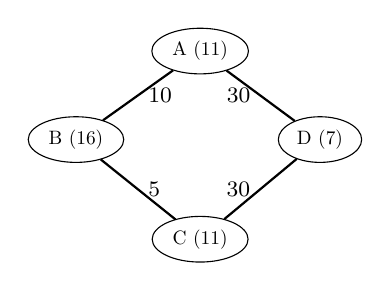
\begin{tikzpicture}
\usetikzlibrary{arrows}
\usetikzlibrary{shapes}
\tikzstyle{every node}=[draw, ellipse, minimum size=10pt,align=center,scale=0.7]
\node at (0,0)(1){A (11)};
\node[below left=1cm of 1](2){B (16)};
\node[below right=1cm of 1](4){D (7)};
\node[below=1.8cm of 1](3){C (11)};
\path[every node/.style={font=\footnotesize},thick]
    (1) edge node[right] {10} (2)
	edge node[left] {30} (4)
    (2) edge node[right] {5} (3)
    (4) edge node[left] {30} (3);
\end{tikzpicture}
  \subcaption{Physical Network}\label{fig:Physical}
  \end{subfigure}  
  \begin{subfigure}[b]{0.53\linewidth}
  \centering
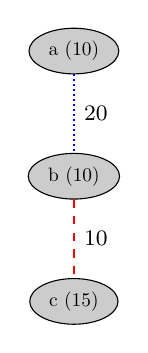
\begin{tikzpicture}
\usetikzlibrary{arrows}
\usetikzlibrary{shapes}
\tikzstyle{every node}=[draw, ellipse, fill=gray!40, minimum size=10pt, align=center, scale=0.7]
\node at (0,0)(1){a (10)};
\node[below=1cm of 1](2){b (10)};
\node[below=1cm of 2](3){c (15)};
\path[every node/.style={font=\footnotesize},thick]
    (1) edge[blue,densely dotted] node[right,color=black] {20} (2)
    (2) edge[red,thick,dashed] node[right,color=black] {10} (3);
\end{tikzpicture}
  \subcaption{Virtual Network}\label{fig:Virtual}
  \end{subfigure}   
  \caption{An input instance for the VNEP.}\label{fig:input}   
\end{figure}
\end{frame}
%---------------------------
\begin{frame}
\frametitle{Virtual Network Embedding Problem}
\begin{figure}
  \centering
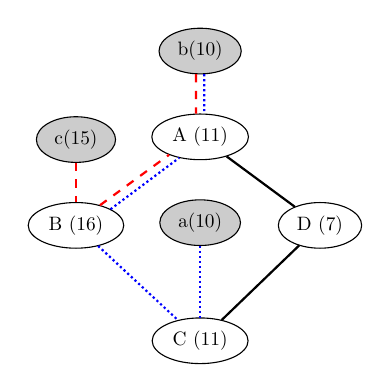
\begin{tikzpicture}
\usetikzlibrary{arrows}
\usetikzlibrary{shapes}
\tikzstyle{every node}=[draw, ellipse, minimum size=10pt,align=center,scale=0.7]
\node[fill=gray!40] at (0,0)(6){b(10)};
\node[below=0.5cm of 6] (1){A (11)};
\node[below left=1cm of 1](2){B (16)};
\node[below right=1cm of 1](4){D (7)};
\node[below=2cm of 1](3){C (11)};
\node[fill=gray!40, below=0.5cm of 1] (5){a(10)};
\node[fill=gray!40, above=0.5cm of 2] (7){c(15)};
\path[every node/.style={font=\footnotesize},thick]
    (5) edge[blue,densely dotted] node [] {} (3)
    (7) edge[red,dashed] node [] {} (2)
    (1) edge node [] {} (4)
    (2) edge[blue,densely dotted] node [] {} (3)
    (4) edge node [] {} (3);
  \draw[blue,thick,densely dotted] (2.25) -- (1.-135);
  \draw[red,thick,dashed] (2.40) -- (1.-150);
  \draw[blue,thick,densely dotted] (6.-80) -- (1.80);
  \draw[red,thick,dashed] (6.-100) -- (1.100);
\end{tikzpicture}
  \caption{Optimal solution for example instance - Cost = 40 + 10 = 50}
\end{figure}
\end{frame}
%---------------------------
\begin{frame}
\frametitle{Path Splitting}
Introduced by (YU et al., 2008)
\begin{figure}
  \centering
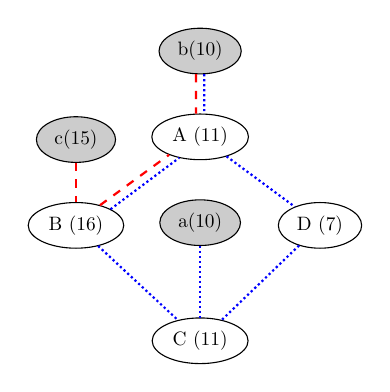
\begin{tikzpicture}
\usetikzlibrary{arrows}
\usetikzlibrary{shapes}
\tikzstyle{every node}=[draw, ellipse, minimum size=10pt,align=center,scale=0.7]
\node[fill=gray!40] at (0,0)(6){b(10)};
\node[below=0.5cm of 6] (1){A (11)};
\node[below left=1cm of 1](2){B (16)};
\node[below right=1cm of 1](4){D (7)};
\node[below=2cm of 1](3){C (11)};
\node[fill=gray!40, below=0.5cm of 1] (5){a(10)};
\node[fill=gray!40, above=0.5cm of 2] (7){c(15)};
\path[every node/.style={font=\footnotesize},thick]
    (5) edge[blue,densely dotted] node [] {} (3)
    (7) edge[red,dashed] node [] {} (2)
    (1) edge[blue,densely dotted] node {} (4)
    (2) edge[blue,densely dotted] node [] {} (3)
    (4) edge[blue,densely dotted] node [] {} (3);
  \draw[blue,thick,densely dotted] (2.25) -- (1.-135);
  \draw[red,thick,dashed] (2.40) -- (1.-150);
  \draw[blue,thick,densely dotted] (6.-80) -- (1.80);
  \draw[red,thick,dashed] (6.-100) -- (1.100);
\end{tikzpicture}
\end{figure}
\pause
\begin{itemize}
  \item Lack of hardware support
  \item Some applications do not allow it
\end{itemize}
\end{frame}
%---------------------------
\section{Related Work}
\begin{frame}
\frametitle{Related Work}
\pause
\begin{enumerate}
  \item Heuristic algorithms (ZHU; AMMAR, 2006; LU; TURNER, 2006), (FAN; AMMAR, 2006), (YU et al., 2008), (LISCHKA; KARL, 2009)
  \item Heuristic algorithm based on LP (CHOWDHURY; RAHMAN; BOUTABA, 2009)
  \item Exact Algorithms based on LP (HOUIDI et al., 2011), (GUERZONI et al., 2014)
  \item Column generation algorithms (JARRAY; KARMOUCH, 2012), (HU; WANG; CAO, 2013)
\end{enumerate}
\end{frame}
%---------------------------
\section{Complexity}
\begin{frame}
\frametitle{Finding a feasible solution for VNEP is NP-Complete}
\pause
\begin{theorem} \label{th:npcomplete}
  VNEP* is an NP-Complete problem.
\end{theorem}

\begin{itemize}
  \item VNEP* is NP (checking is $O(|E^V||E^S|)$)
  \item VNEP* is NP-Hard
  \begin{itemize}
    \item Transformation $\phi$ ($BPP\le_P VNEP^*$)
    \item $\phi$ is polynomial
  \end{itemize}
\end{itemize}
\end{frame}
%---------------------------
\begin{comment}
\begin{frame}
\frametitle{VNEP* is NP}
\begin{itemize}
  \item node mapping
  \begin{itemize}
    \item Every virtual node is mapped to a different physical node
    \item All physical nodes have enough resources to host the virtual nodes mapped to them
  \end{itemize}
  \item link mapping
  \begin{itemize}
    \item Every virtual link is mapped to a valid path in the physical graph between the physical links for which their endpoints were mapped
    \item Every physical link has enough capacity to host its virtual links
  \end{itemize}
\end{itemize}
\end{frame}
\end{comment}
%---------------------------
\begin{frame}
\frametitle{Transformation $\phi$}
$ B = 8; w = \{3,4,8\}; k = 2$

\pause

\begin{columns}
\begin{column}{0.4\textwidth}
\begin{figure}
  \centering
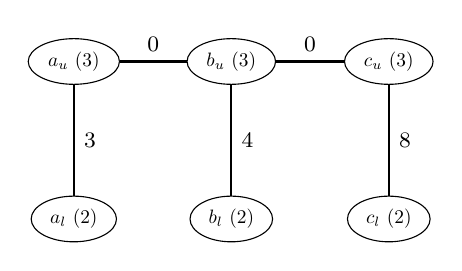
\begin{tikzpicture}
\usetikzlibrary{arrows}
\usetikzlibrary{shapes}
\usetikzlibrary{graphs}
\tikzstyle{every node}=[draw, ellipse, minimum size=10pt,align=center,scale=0.7]
\node at (0,2)(1){$a_{u}$ (3)};
\node at (2,2)(2){$b_{u}$ (3)};
\node at (4,2)(3){$c_{u}$ (3)};
\node at (0,0)(8){$a_{l}$ (2)};
\node at (2,0)(9){$b_{l}$ (2)};
\node at (4,0)(10){$c_{l}$ (2)};
\path[every node/.style={font=\footnotesize},thick]
    (1) edge node[right] {3} (8)
    (2) edge node[right] {4} (9)
    (3) edge node[right] {8} (10)
    (1) edge node[above] {0} (2)
    (2) edge node[above] {0} (3);
\end{tikzpicture}
\caption{Virtual Graph}
\end{figure}
\end{column}
\pause
\begin{column}{0.4\textwidth}
\begin{figure}
  \centering
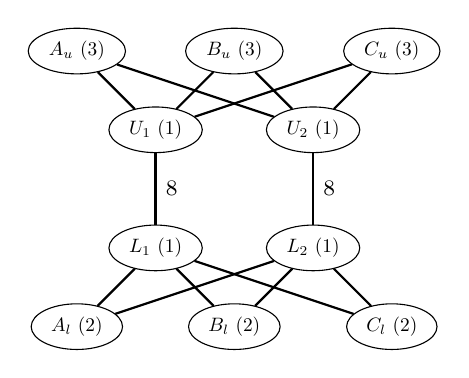
\begin{tikzpicture}
\usetikzlibrary{arrows}
\usetikzlibrary{shapes}
\usetikzlibrary{graphs}
\tikzstyle{every node}=[draw, ellipse, minimum size=10pt,align=center,scale=0.7]
\node at (0,3.5)(1){$A_{u}$ (3)};
\node at (2,3.5)(2){$B_{u}$ (3)};
\node at (4,3.5)(3){$C_{u}$ (3)};
\node at (1,2.5)(4){$U_{1}$ (1)};
\node at (3,2.5)(5){$U_{2}$ (1)};
\node at (1,1)(6){$L_{1}$ (1)};
\node at (3,1)(7){$L_{2}$ (1)};
\node at (0,0)(8){$A_{l}$ (2)};
\node at (2,0)(9){$B_{l}$ (2)};
\node at (4,0)(10){$C_{l}$ (2)};
\path[every node/.style={font=\footnotesize},thick]
    (1) edge node[left] {} (4) 
    (1) edge node[right] {} (5)
    (2) edge node[left] {} (4)
    (2) edge node[right] {} (5)
    (3) edge node[left] {} (4)
    (3) edge node[right] {} (5)
    (4) edge node[right] {8} (6)
    (5) edge node[right] {8} (7)
    (8) edge node[right] {} (6)
    (8) edge node[right] {} (7)
    (9) edge node[left] {} (6)
    (9) edge node[right] {} (7)
    (10) edge node[left] {} (6)
    (10) edge node[right] {} (7);
\end{tikzpicture}
  \caption{Substrate Graph} 
\end{figure}
\end{column}

\end{columns}

\pause

$\phi$ is polynomial.

\end{frame}
%---------------------------
\section{Models}
\begin{frame}
\frametitle{Compact Model}
\pause
{
\begin{columns}
\begin{column}{0.35\textwidth}
  \begin{itemize}
    \item $x_{vs}$ - virtual node $v$ is mapped into physical node $s$.
    \item $y_{vwst}$ - virtual link $(v,w)$ is mapped into physical edge $(s,t)$.
  \end{itemize}
\end{column}
\pause
\begin{column}{0.7\textwidth}
\tiny
\begin{align}
     \min & \sum\limits_{(s,t) \in E^{S}} \sum\limits_{(v,w) \in E^{V}} B_{vw}~ y_{vwst} & \nonumber \\
    s.t. & \sum\limits_{v \in V^{V}} C_{v} x_{vs} \leq C_{s}                                   & \forall s \in V^{S}  \nonumber \\
         & \sum\limits_{s \in V^{S}} x_{vs} = 1                                                & \forall v \in V^{V}  \nonumber\\
         & \sum\limits_{v \in V^{V}} x_{vs} \leq 1                                             & \forall s \in V^{S} \nonumber \\
         & \sum\limits_{t \in V^{S}} ( y_{vwst} - y_{vwts}) = x_{vs} - x_{ws} & \forall (v,w) \in E^{V}, \nonumber \\ 
         &                                                                    & s \in V^{S} \nonumber \\
         & \sum\limits_{(v,w) \in E^{V}} B_{vw}  y_{vwst} \leq B_{st}                 & \forall (s,t) \in E^{S} \nonumber \\
         & x_{vs} \in \{0,1\}                                                                  & \forall v \in V^{V}, \nonumber \\
         &                                                                                      & s \in V^{S} \nonumber \\
         & y_{klmn} \in \{0,1\}                                                         & \forall (k,l) \in E^{V}, \nonumber \\
         &                                                                                 & (m,n) \in E^{S} \nonumber  
\end{align} 
\end{column}
\end{columns}
}
\end{frame}
\begin{frame}
\frametitle{Compact Model}
{
\begin{columns}
\begin{column}{0.35\textwidth}
\begin{proposition}
There is always a solution with cost zero to the compact model.
\end{proposition}
\end{column}
\begin{column}{0.7\textwidth}
\tiny
\begin{align}
     \min & \sum\limits_{(s,t) \in E^{S}} \sum\limits_{(v,w) \in E^{V}} B_{vw}~ y_{vwst} & \nonumber \\
    s.t. & \sum\limits_{v \in V^{V}} C_{v} x_{vs} \leq C_{s}                                   & \forall s \in V^{S}  \nonumber \\
         & \sum\limits_{s \in V^{S}} x_{vs} = 1                                                & \forall v \in V^{V}  \nonumber\\
         & \sum\limits_{v \in V^{V}} x_{vs} \leq 1                                             & \forall s \in V^{S} \nonumber \\
         & \sum\limits_{t \in V^{S}} ( y_{vwst} - y_{vwts}) = x_{vs} - x_{ws} & \forall (v,w) \in E^{V}, \nonumber \\ 
         &                                                                    & s \in V^{S} \nonumber \\
         & \sum\limits_{(v,w) \in E^{V}} B_{vw}  y_{vwst} \leq B_{st}                 & \forall (s,t) \in E^{S} \nonumber \\
         & x_{vs} \in \{0,1\}                                                                  & \forall v \in V^{V}, \nonumber \\
         &                                                                                      & s \in V^{S} \nonumber \\
         & y_{klmn} \in \{0,1\}                                                         & \forall (k,l) \in E^{V}, \nonumber \\
         &                                                                                 & (m,n) \in E^{S} \nonumber  
\end{align} 
\end{column}
\end{columns}
}
\end{frame}
%---------------------------
\begin{frame}
\frametitle{Path-based Model}
{
\begin{columns}
\begin{column}{0.35\textwidth}
  \begin{itemize}
    \item $x_{v,s}$ - virtual node $v$ is mapped into physical node $s$.
    \item $z_{p}$ - path $p$ is used
  \end{itemize}
\end{column}
\pause
\begin{column}{0.45\textwidth}
\tiny
\begin{align}
  \min  & \sum\limits_{k \in E^{V}}\sum\limits_{p \in P^k}  c_{p} B_k z_{p} \nonumber \\
        & \sum\limits_{s \in V^{S}} x_{v,s} = 1                                  & \forall v \in V^{V} \nonumber  \\
        & \sum\limits_{v \in V^{V}} x_{v,s} \leq 1                               & \forall s \in V^{S} \nonumber \\
        & \sum\limits_{p \in P^{k}} z_{p} = 1                                    & \forall k \in E^{V} \nonumber \\
        & \sum\limits_{k \in E^{V}}\sum\limits_{p \in P^{k}} \delta_{e,p} B_{k} z_{p} \leq B_{e} & \forall e \in E^{S} \nonumber \\
        &  \sum\limits_{k \in E^{V}}\sum\limits_{p \in P^k : (v,s) \in p} z_{p} \leq M x_{v,s} & \forall v \in V^{V}, s \in V^{S} \nonumber\\
        & 0 \leq x_{v,s} \leq 1  & \forall v \in V^{V}, s \in V^{S} \nonumber \\
        & 0 \leq z_{p}   \leq 1  & \forall p \in {P} \nonumber
\end{align}
\end{column}
\end{columns}
}
\end{frame}
%----------------------------------------
\begin{frame}
  \frametitle{Path-based Model}
  \begin{itemize}
    \item Large Model cannot be solved with simplex algorithm
    \item Column generation solves linear relaxation of Path-based model
  \end{itemize}
\end{frame}
\section{Column Generation}
\begin{frame}
  \frametitle{Column Generation Algorithm}
  \pause
\begin{enumerate}
	\item Find an initial set of columns
	\item Solve Restricted Master Problem
	\item Solve pricing problem
	\item If no columns are found, terminate, otherwise add new columns to RMP and goto~2
\end{enumerate}
\end{frame}
%---------------------------
\begin{frame}
  \frametitle{Pricing Problem}
  \begin{itemize}
    \item Pricing - find a column that can improve the current RMP solution
    \item Find the column with the smallest \textbf{reduced cost}
  \end{itemize}
  \pause


\begin{columns}
\begin{column}{0.4\textwidth}
  \scriptsize
  \begin{align}
        & \sum\limits_{p \in P^{k}} z_{p} = 1                                    & \forall k \in E^{V} \nonumber \\
        & \sum\limits_{k \in E^{V}}\sum\limits_{p \in P^{k}} \delta_{e,p} B_{k} z_{p} \leq B_{e} & \forall e \in E^{S} \nonumber \\
        &  \sum\limits_{k \in E^{V}}\sum\limits_{p \in P^k : (v,s) \in p} z_{p} \leq M x_{v,s} & \forall v \in V^{V} \nonumber \\
        & & s \in V^{S} \nonumber
  \end{align}
\end{column}

\pause

\begin{column}{0.4\textwidth}
  \scriptsize
  \centering
  \begin{align}
    r_{p} = c_{p} B_{k} - \lambda_{k} - \sum\limits_{e \in p : e \in E^S} B_{k} y_{e}  - \sum\limits_{(v,s) \in p : (v,s) \notin E^S} \pi_{v,s}  \nonumber
  \end{align}

  \pause

  \begin{align}
    r_{p} = \sum\limits_{e \in p : e \in E^S} B_{k} (1 - y_{e}) - \sum\limits_{e \in p : e \notin E^S} \pi_e - \lambda_{k} \nonumber
  \end{align}

  \pause

  \begin{align}
    \min_{ \forall k \in E^{V}, \forall p \in P^{k}}  \quad  \sum\limits_{e \in p : e \in E^S} B_{k} (1 - y_{e}) - \sum\limits_{e \in p : e \notin E^S} \pi_{e}-\lambda_{k} \nonumber
  \end{align}
\end{column}
\end{columns}

\end{frame}
%---------------------------
\begin{frame}
\frametitle{The Auxiliary Graph}
\begin{figure}
  \centering
  \begin{subfigure}[b]{0.4\linewidth}
  \centering    
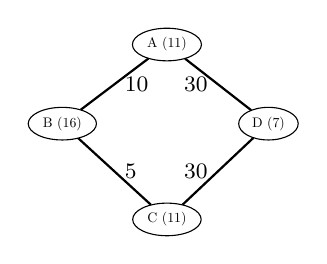
\begin{tikzpicture}
\usetikzlibrary{arrows}
\usetikzlibrary{shapes}
\tikzstyle{every node}=[draw, ellipse, minimum size=5pt,align=center,scale=0.5]
\node at (0,0)(1){A (11)};
\node[below left=1cm of 1](2){B (16)};
\node[below right=1cm of 1](4){D (7)};
\node[below=1.8cm of 1](3){C (11)};
\path[every node/.style={font=\footnotesize},thick]
    (1) edge node[right] {10} (2)
	edge node[left] {30} (4)
    (2) edge node[right] {5} (3)
    (4) edge node[left] {30} (3);
\end{tikzpicture}
  \end{subfigure}  
  \begin{subfigure}[b]{0.3\linewidth}
  \centering
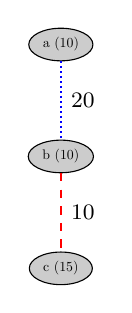
\begin{tikzpicture}
\usetikzlibrary{arrows}
\usetikzlibrary{shapes}
\tikzstyle{every node}=[draw, ellipse, fill=gray!40, minimum size=5pt, align=center, scale=0.5]
\node at (0,0)(1){a (10)};
\node[below=1cm of 1](2){b (10)};
\node[below=1cm of 2](3){c (15)};
\path[every node/.style={font=\footnotesize},thick]
    (1) edge[blue,densely dotted] node[right,color=black] {20} (2)
    (2) edge[red,thick,dashed] node[right,color=black] {10} (3);
\end{tikzpicture}
  \end{subfigure}   
  \begin{subfigure}[b]{0.33\linewidth}
  \centering
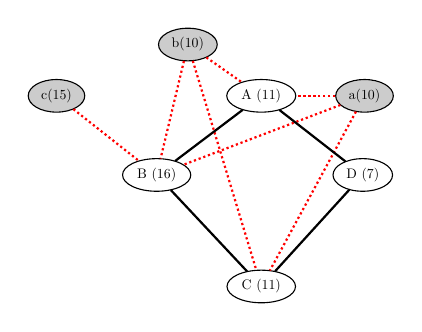
\begin{tikzpicture}
\usetikzlibrary{arrows}
\usetikzlibrary{shapes}
\tikzstyle{every node}=[draw, ellipse, minimum size=5pt,align=center,scale=0.5]
\node[fill=gray!40] at (0,0)(6){b(10)};
\node[below right=0.5cm of 6] (1){A (11)};
\node[below left=1cm of 1](2){B (16)};
\node[below right=1cm of 1](4){D (7)};
\node[below=2cm of 1](3){C (11)};
\node[fill=gray!40, right=0.5cm of 1] (5){a(10)};
\node[fill=gray!40, above left=1cm of 2] (7){c(15)};
\path[every node/.style={font=\sffamily\small},thick]
    (5) edge[red,densely dotted] node [] {} (1)
	edge[red,densely dotted] node [] {} (2)
	edge[red,densely dotted] node [] {} (3)
    (6) edge[red,densely dotted] node [] {} (1)
	edge[red,densely dotted] node [] {} (2)
	edge[red,densely dotted] node [] {} (3)
    (7) edge[red,densely dotted] node [] {} (2)
    (1) edge node [] {} (4)
    (2) edge node [] {} (3)
	edge node [] {} (1)
    (4) edge node [] {} (3);
\end{tikzpicture}
\end{subfigure}
\end{figure}
\end{frame}
%---------------------------
\begin{frame}
\frametitle{Solving the Pricing Problem}
  Find column with the smallest reduced cost

  \begin{figure}
    \centering
    \includegraphics[scale=0.4]{redcost1.png}
  \end{figure}

\end{frame}
\begin{frame}
\frametitle{Pricing}
  The cost of a path in the auxiliary graph is its reduced cost

  \begin{figure}
    \centering
    \includegraphics[scale=0.4]{redcost2.png}
  \end{figure}

\end{frame}
%---------------------------
\begin{frame}
\frametitle{Valid Paths}
\begin{figure}[h]
  \centering
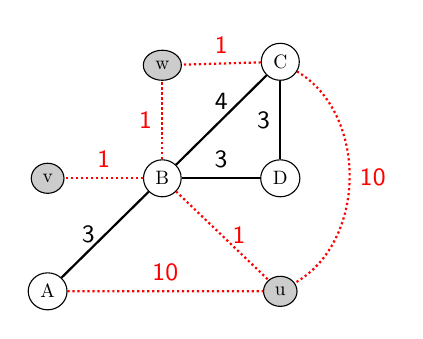
\begin{tikzpicture}
\usetikzlibrary{arrows}
\usetikzlibrary{shapes}
\tikzstyle{every node}=[draw, ellipse, minimum size=10pt,align=center,scale=0.7]
\node at (0,0)(B){B};
\node[right=1cm of B](D){D};
\node[fill=gray!40,left=1cm of B](v){v};
\node[below=1cm of v](A){A};
\node[above=1cm of D] (C){C};
\node[fill=gray!40,above=1cm of B] (w){w};
\node[fill=gray!40, below=1cm of D](u){u};
\path[every node/.style={font=\sffamily\small},thick]
    (A) edge[red,densely dotted] node [above] {10} (u)
    (B) edge node [left, above] {4} (C)
  edge[red,densely dotted] node [left] {1} (w)
	edge node [above] {3} (D)
	edge node [left] {3} (A)
	edge[red,densely dotted] node [right] {1} (u)
	edge[red,densely dotted] node [above] {1} (v)
    (C) edge node [left] {3} (D)
  edge[red,densely dotted] node [above] {1} (w)
  edge[red,densely dotted, bend left=60] node [right] {10} (u);
\end{tikzpicture}
\end{figure}
\end{frame}
%---------------------------
\begin{frame}
\frametitle{Valid Paths}
\begin{figure}[h]
  \centering
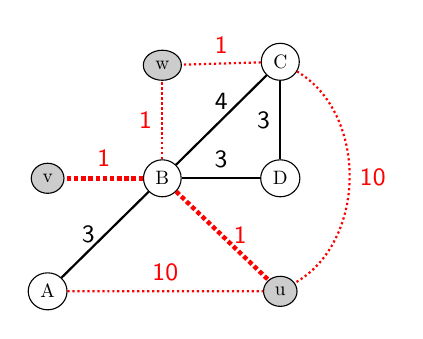
\begin{tikzpicture}
\usetikzlibrary{arrows}
\usetikzlibrary{shapes}
\tikzstyle{every node}=[draw, ellipse, minimum size=10pt,align=center,scale=0.7]
\node at (0,0)(B){B};
\node[right=1cm of B](D){D};
\node[fill=gray!40,left=1cm of B](v){v};
\node[below=1cm of v](A){A};
\node[above=1cm of D] (C){C};
\node[fill=gray!40,above=1cm of B] (w){w};
\node[fill=gray!40, below=1cm of D](u){u};
\path[every node/.style={font=\sffamily\small},thick]
    (A) edge[red,densely dotted] node [above] {10} (u)
    (B) edge node [left, above] {4} (C)
  edge[red,densely dotted] node [left] {1} (w)
	edge node [above] {3} (D)
	edge node [left] {3} (A)
	edge[red,densely dotted,ultra thick] node [right] {1} (u)
	edge[red,densely dotted,ultra thick] node [above] {1} (v)
    (C) edge node [left] {3} (D)
  edge[red,densely dotted] node [above] {1} (w)
  edge[red,densely dotted, bend left=60] node [right] {10} (u);
\end{tikzpicture}
\end{figure}
\begin{center}
  cost = 2
\end{center}
\end{frame}
%---------------------------
\begin{frame}
\frametitle{Valid Paths}
\begin{figure}[h]
  \centering
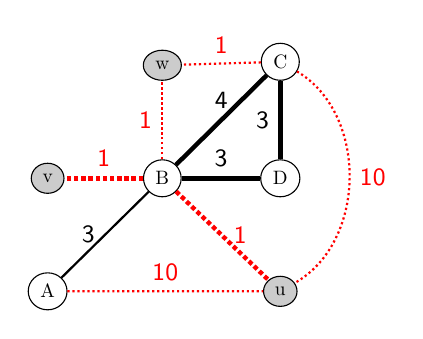
\begin{tikzpicture}
\usetikzlibrary{arrows}
\usetikzlibrary{shapes}
\tikzstyle{every node}=[draw, ellipse, minimum size=10pt,align=center,scale=0.7]
\node at (0,0)(B){B};
\node[right=1cm of B](D){D};
\node[fill=gray!40,left=1cm of B](v){v};
\node[below=1cm of v](A){A};
\node[above=1cm of D] (C){C};
\node[fill=gray!40,above=1cm of B] (w){w};
\node[fill=gray!40, below=1cm of D](u){u};
\path[every node/.style={font=\sffamily\small},thick]
    (A) edge[red,densely dotted] node [above] {10} (u)
    (B) edge[ultra thick] node [left, above] {4} (C)
  edge[red,densely dotted] node [left] {1} (w)
  edge[ultra thick] node [above] {3} (D)
	edge node [left] {3} (A)
	edge[red,densely dotted,ultra thick] node [right] {1} (u)
	edge[red,densely dotted,ultra thick] node [above] {1} (v)
  (C) edge[ultra thick] node [left] {3} (D)
  edge[red,densely dotted] node [above] {1} (w)
  edge[red,densely dotted, bend left=60] node [right] {10} (u);
\end{tikzpicture}
\end{figure}
\begin{center}
  cost = 12
\end{center}
\end{frame}
%---------------------------
\begin{frame}
\frametitle{Valid Paths}
\begin{figure}[h]
  \centering
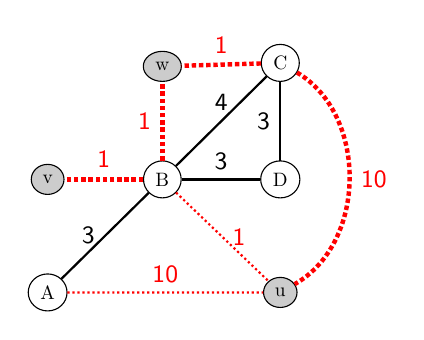
\begin{tikzpicture}
\usetikzlibrary{arrows}
\usetikzlibrary{shapes}
\tikzstyle{every node}=[draw, ellipse, minimum size=10pt,align=center,scale=0.7]
\node at (0,0)(B){B};
\node[right=1cm of B](D){D};
\node[fill=gray!40,left=1cm of B](v){v};
\node[below=1cm of v](A){A};
\node[above=1cm of D] (C){C};
\node[fill=gray!40,above=1cm of B] (w){w};
\node[fill=gray!40, below=1cm of D](u){u};
\path[every node/.style={font=\sffamily\small},thick]
    (A) edge[red,densely dotted] node [above] {10} (u)
    (B) edge node [left, above] {4} (C)
  edge[red,densely dotted,ultra thick] node [left] {1} (w)
	edge node [above] {3} (D)
	edge node [left] {3} (A)
	edge[red,densely dotted] node [right] {1} (u)
	edge[red,densely dotted,ultra thick] node [above] {1} (v)
    (C) edge node [left] {3} (D)
  edge[red,densely dotted,ultra thick] node [above] {1} (w)
  edge[red,densely dotted,ultra thick,bend left=60] node [right] {10} (u);
\end{tikzpicture}
\end{figure}
\begin{center}
  cost = 13
\end{center}
\end{frame}
%---------------------------
\begin{frame}
\frametitle{Pricing}
\begin{figure}[h]
  \centering
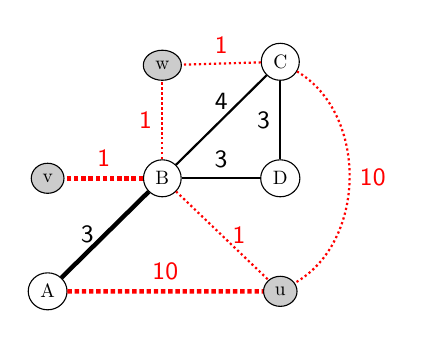
\begin{tikzpicture}
\usetikzlibrary{arrows}
\usetikzlibrary{shapes}
\tikzstyle{every node}=[draw, ellipse, minimum size=10pt,align=center,scale=0.7]
\node at (0,0)(B){B};
\node[right=1cm of B](D){D};
\node[fill=gray!40,left=1cm of B](v){v};
\node[below=1cm of v](A){A};
\node[above=1cm of D] (C){C};
\node[fill=gray!40,above=1cm of B] (w){w};
\node[fill=gray!40, below=1cm of D](u){u};
\path[every node/.style={font=\sffamily\small},thick]
    (A) edge[red,densely dotted,ultra thick] node [above] {10} (u)
    (B) edge node [left, above] {4} (C)
  edge[red,densely dotted] node [left] {1} (w)
	edge node [above] {3} (D)
  edge[ultra thick] node [left] {3} (A)
	edge[red,densely dotted] node [right] {1} (u)
	edge[red,densely dotted,ultra thick] node [above] {1} (v)
    (C) edge node [left] {3} (D)
  edge[red,densely dotted] node [above] {1} (w)
  edge[red,densely dotted, bend left=60] node [right] {10} (u);
\end{tikzpicture}
\end{figure}
\begin{center}
  cost = 14
\end{center}
\end{frame}
%---------------------------
\begin{frame}
\frametitle{Modified Dijkstra's Algorithm}
\begin{figure}[h]
  \centering
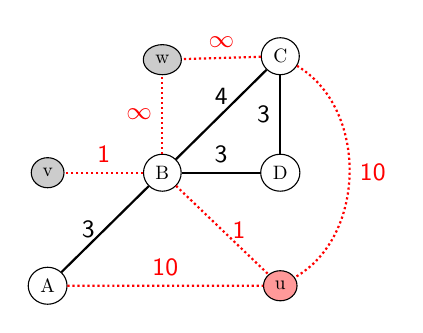
\begin{tikzpicture}
\usetikzlibrary{arrows}
\usetikzlibrary{shapes}
\tikzstyle{every node}=[draw, ellipse, minimum size=10pt,align=center,scale=0.7]
\node at (0,0)(B){B};
\node[right=1cm of B](D){D};
\node[fill=gray!40,left=1cm of B](v){v};
\node[below=1cm of v](A){A};
\node[above=1cm of D] (C){C};
\node[fill=gray!40,above=1cm of B] (w){w};
\node[fill=red!40, below=1cm of D](u){u};
\path[every node/.style={font=\sffamily\small},thick]
    (A) edge[red,densely dotted] node [above] {10} (u)
    (B) edge node [left, above] {4} (C)
  edge[red,densely dotted] node [left] {$\infty$} (w)
	edge node [above] {3} (D)
	edge node [left] {3} (A)
	edge[red,densely dotted] node [right] {1} (u)
	edge[red,densely dotted] node [above] {1} (v)
    (C) edge node [left] {3} (D)
  edge[red,densely dotted] node [above] {$\infty$} (w)
  edge[red,densely dotted, bend left=60] node [right] {10} (u);
\end{tikzpicture}
\end{figure}
\begin{equation}
  Q = \{(A,A,10); (B,B,1); (C,C,10)\} \nonumber
\end{equation}
\end{frame}
\begin{frame}
\frametitle{Modified Dijkstra's Algorithm}
\begin{figure}[h]
  \centering
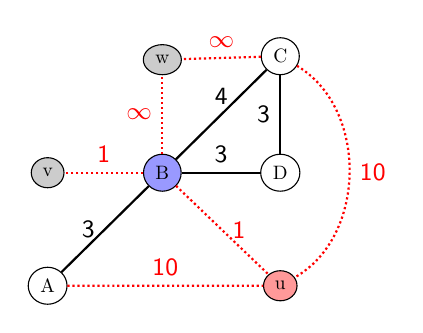
\begin{tikzpicture}
\usetikzlibrary{arrows}
\usetikzlibrary{shapes}
\tikzstyle{every node}=[draw, ellipse, minimum size=10pt,align=center,scale=0.7]
\node[fill=blue!40] at (0,0)(B){B};
\node[right=1cm of B](D){D};
\node[fill=gray!40,left=1cm of B](v){v};
\node[below=1cm of v](A){A};
\node[above=1cm of D] (C){C};
\node[fill=gray!40,above=1cm of B] (w){w};
\node[fill=red!40, below=1cm of D](u){u};
\path[every node/.style={font=\sffamily\small},thick]
    (A) edge[red,densely dotted] node [above] {10} (u)
    (B) edge node [left, above] {4} (C)
  edge[red,densely dotted] node [left] {$\infty$} (w)
	edge node [above] {3} (D)
	edge node [left] {3} (A)
	edge[red,densely dotted] node [right] {1} (u)
	edge[red,densely dotted] node [above] {1} (v)
    (C) edge node [left] {3} (D)
  edge[red,densely dotted] node [above] {$\infty$} (w)
  edge[red,densely dotted, bend left=60] node [right] {10} (u);
\end{tikzpicture}
\end{figure}
\begin{equation}
  Q = \{(A,A,10); (C,C,10); (A,B,4); (C,B,5); (D,B,4)\} \nonumber
\end{equation}
\end{frame}
\begin{frame}
\frametitle{Modified Dijkstra's Algorithm}
\begin{figure}[h]
  \centering
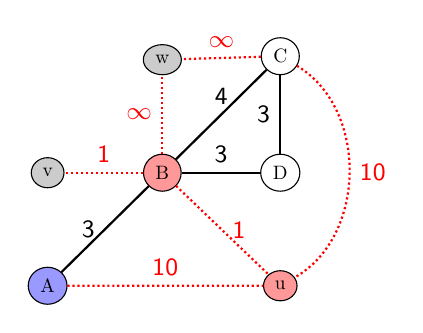
\begin{tikzpicture}
\usetikzlibrary{arrows}
\usetikzlibrary{shapes}
\tikzstyle{every node}=[draw, ellipse, minimum size=10pt,align=center,scale=0.7]
\node[fill=red!40] at (0,0)(B){B};
\node[right=1cm of B](D){D};
\node[fill=gray!40,left=1cm of B](v){v};
\node[fill=blue!40,below=1cm of v](A){A};
\node[above=1cm of D] (C){C};
\node[fill=gray!40,above=1cm of B] (w){w};
\node[fill=red!40, below=1cm of D](u){u};
\path[every node/.style={font=\sffamily\small},thick]
    (A) edge[red,densely dotted] node [above] {10} (u)
    (B) edge node [left, above] {4} (C)
  edge[red,densely dotted] node [left] {$\infty$} (w)
	edge node [above] {3} (D)
	edge node [left] {3} (A)
	edge[red,densely dotted] node [right] {1} (u)
	edge[red,densely dotted] node [above] {1} (v)
    (C) edge node [left] {3} (D)
  edge[red,densely dotted] node [above] {$\infty$} (w)
  edge[red,densely dotted, bend left=60] node [right] {10} (u);
\end{tikzpicture}
\end{figure}
\begin{equation}
  Q = \{(A,A,10); (C,C,10); (C,B,5); (D,B,4)\} \nonumber
\end{equation}
\end{frame}
\begin{frame}
\frametitle{Modified Dijkstra's Algorithm}
\begin{figure}[h]
  \centering
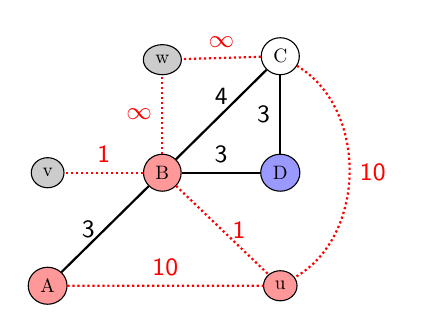
\begin{tikzpicture}
\usetikzlibrary{arrows}
\usetikzlibrary{shapes}
\tikzstyle{every node}=[draw, ellipse, minimum size=10pt,align=center,scale=0.7]
\node[fill=red!40] at (0,0)(B){B};
\node[fill=blue!40,right=1cm of B](D){D};
\node[fill=gray!40,left=1cm of B](v){v};
\node[fill=red!40,below=1cm of v](A){A};
\node[above=1cm of D] (C){C};
\node[fill=gray!40,above=1cm of B] (w){w};
\node[fill=red!40, below=1cm of D](u){u};
\path[every node/.style={font=\sffamily\small},thick]
    (A) edge[red,densely dotted] node [above] {10} (u)
    (B) edge node [left, above] {4} (C)
  edge[red,densely dotted] node [left] {$\infty$} (w)
	edge node [above] {3} (D)
	edge node [left] {3} (A)
	edge[red,densely dotted] node [right] {1} (u)
	edge[red,densely dotted] node [above] {1} (v)
    (C) edge node [left] {3} (D)
  edge[red,densely dotted] node [above] {$\infty$} (w)
  edge[red,densely dotted, bend left=60] node [right] {10} (u);
\end{tikzpicture}
\end{figure}
\begin{equation}
  Q = \{(A,A,10);(C,C,10);(C,B,5)\} \nonumber
\end{equation}
\end{frame}
\begin{frame}
\frametitle{Modified Dijkstra's Algorithm}
\begin{figure}[h]
  \centering
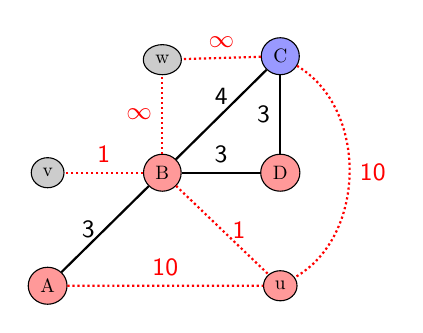
\begin{tikzpicture}
\usetikzlibrary{arrows}
\usetikzlibrary{shapes}
\tikzstyle{every node}=[draw, ellipse, minimum size=10pt,align=center,scale=0.7]
\node[fill=red!40] at (0,0)(B){B};
\node[fill=red!40,right=1cm of B](D){D};
\node[fill=gray!40,left=1cm of B](v){v};
\node[fill=red!40,below=1cm of v](A){A};
\node[fill=blue!40,above=1cm of D] (C){C};
\node[fill=gray!40,above=1cm of B] (w){w};
\node[fill=red!40, below=1cm of D](u){u};
\path[every node/.style={font=\sffamily\small},thick]
    (A) edge[red,densely dotted] node [above] {10} (u)
    (B) edge node [left, above] {4} (C)
  edge[red,densely dotted] node [left] {$\infty$} (w)
	edge node [above] {3} (D)
	edge node [left] {3} (A)
	edge[red,densely dotted] node [right] {1} (u)
	edge[red,densely dotted] node [above] {1} (v)
    (C) edge node [left] {3} (D)
  edge[red,densely dotted] node [above] {$\infty$} (w)
  edge[red,densely dotted, bend left=60] node [right] {10} (u);
\end{tikzpicture}
\end{figure}
\begin{equation}
  Q = \{(A,A,10);(C,C,10)\} \nonumber
\end{equation}
\end{frame}
\begin{frame}
\frametitle{Modified Dijkstra's Algorithm}
\begin{figure}[h]
  \centering
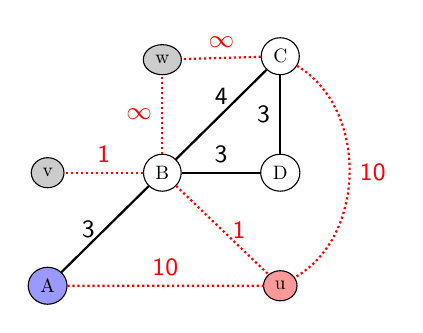
\begin{tikzpicture}
\usetikzlibrary{arrows}
\usetikzlibrary{shapes}
\tikzstyle{every node}=[draw, ellipse, minimum size=10pt,align=center,scale=0.7]
\node[fill=white!40] at (0,0)(B){B};
\node[fill=white!40,right=1cm of B](D){D};
\node[fill=gray!40,left=1cm of B](v){v};
\node[fill=blue!40,below=1cm of v](A){A};
\node[fill=white!40,above=1cm of D] (C){C};
\node[fill=gray!40,above=1cm of B] (w){w};
\node[fill=red!40, below=1cm of D](u){u};
\path[every node/.style={font=\sffamily\small},thick]
    (A) edge[red,densely dotted] node [above] {10} (u)
    (B) edge node [left, above] {4} (C)
  edge[red,densely dotted] node [left] {$\infty$} (w)
	edge node [above] {3} (D)
	edge node [left] {3} (A)
	edge[red,densely dotted] node [right] {1} (u)
	edge[red,densely dotted] node [above] {1} (v)
    (C) edge node [left] {3} (D)
  edge[red,densely dotted] node [above] {$\infty$} (w)
  edge[red,densely dotted, bend left=60] node [right] {10} (u);
\end{tikzpicture}
\end{figure}
\begin{equation}
  Q = \{(C,C,10);(B,A,13)\} \nonumber
\end{equation}
\end{frame}
\begin{frame}
\frametitle{Modified Dijkstra's Algorithm}
\begin{figure}[h]
  \centering
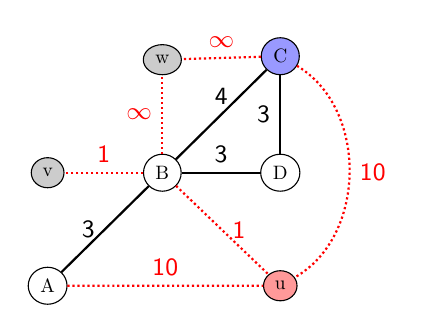
\begin{tikzpicture}
\usetikzlibrary{arrows}
\usetikzlibrary{shapes}
\tikzstyle{every node}=[draw, ellipse, minimum size=10pt,align=center,scale=0.7]
\node[fill=white!40] at (0,0)(B){B};
\node[fill=white!40,right=1cm of B](D){D};
\node[fill=gray!40,left=1cm of B](v){v};
\node[fill=white!40,below=1cm of v](A){A};
\node[fill=blue!40,above=1cm of D] (C){C};
\node[fill=gray!40,above=1cm of B] (w){w};
\node[fill=red!40, below=1cm of D](u){u};
\path[every node/.style={font=\sffamily\small},thick]
    (A) edge[red,densely dotted] node [above] {10} (u)
    (B) edge node [left, above] {4} (C)
  edge[red,densely dotted] node [left] {$\infty$} (w)
	edge node [above] {3} (D)
	edge node [left] {3} (A)
	edge[red,densely dotted] node [right] {1} (u)
	edge[red,densely dotted] node [above] {1} (v)
    (C) edge node [left] {3} (D)
  edge[red,densely dotted] node [above] {$\infty$} (w)
  edge[red,densely dotted, bend left=60] node [right] {10} (u);
\end{tikzpicture}
\end{figure}
\begin{equation}
  Q = \{(B,A,13);(D,C,13);(B,C,14)\} \nonumber
\end{equation}
\end{frame}
\begin{frame}
\frametitle{Modified Dijkstra's Algorithm}
\begin{figure}[h]
  \centering
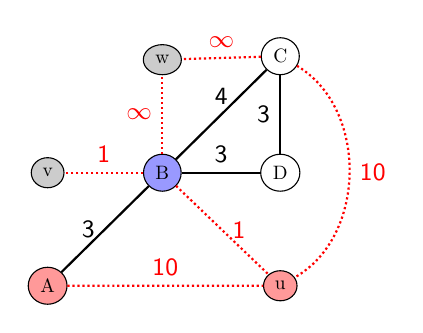
\begin{tikzpicture}
\usetikzlibrary{arrows}
\usetikzlibrary{shapes}
\tikzstyle{every node}=[draw, ellipse, minimum size=10pt,align=center,scale=0.7]
\node[fill=blue!40] at (0,0)(B){B};
\node[fill=white!40,right=1cm of B](D){D};
\node[fill=gray!40,left=1cm of B](v){v};
\node[fill=red!40,below=1cm of v](A){A};
\node[fill=white!40,above=1cm of D] (C){C};
\node[fill=gray!40,above=1cm of B] (w){w};
\node[fill=red!40, below=1cm of D](u){u};
\path[every node/.style={font=\sffamily\small},thick]
    (A) edge[red,densely dotted] node [above] {10} (u)
    (B) edge node [left, above] {4} (C)
  edge[red,densely dotted] node [left] {$\infty$} (w)
	edge node [above] {3} (D)
	edge node [left] {3} (A)
	edge[red,densely dotted] node [right] {1} (u)
	edge[red,densely dotted] node [above] {1} (v)
    (C) edge node [left] {3} (D)
  edge[red,densely dotted] node [above] {$\infty$} (w)
  edge[red,densely dotted, bend left=60] node [right] {10} (u);
\end{tikzpicture}
\end{figure}
\begin{equation}
  Q = \{(D,C,13);(B,C,14);(v,A,14);(C,A,17);(D,A,16)\} \nonumber
\end{equation}
\pause
\ldots
\begin{equation}
  Q = \{(B,C,14);(v,A,14);(v,C,15);(C,A,17);(D,A,16)\} \nonumber
\end{equation}

\end{frame}
%---------------------------
\begin{frame}
\frametitle{Column Generation Algorithm}
\begin{enumerate}
	\item Solve Restricted Master Problem
	\item Build auxiliary graph
	\item For each virtual link $k$
	\item \quad If there exists a path in the auxiliary graph with negative cost, add column to the model
	\item end if no paths were found in this iteration, otherwise goto~2
\end{enumerate}
\end{frame}
%---------------------------
\section{Branch \& Price}
\begin{frame}
\frametitle{Branch \& Price Algorithm}
\pause
\begin{figure}[h]
  \centering
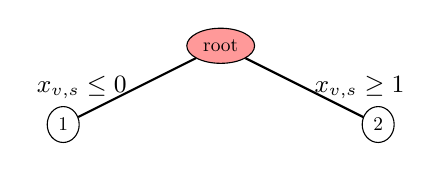
\begin{tikzpicture}
\usetikzlibrary{arrows}
\usetikzlibrary{shapes}
\tikzstyle{every node}=[draw, ellipse, minimum size=10pt,align=center,scale=0.7]
\node [fill=red!40] at ( 0, 0)(0) {root};
\node at (-2,-1)(1) {1};
\node at ( 2,-1)(2) {2};
\path[every node/.style={font=\sffamily\small},thick]
  (0) edge [] node [left] {$ x_{v,s} \leq 0$} (1)
  (0) edge [] node [right] {$ x_{v,s} \geq 1$} (2);
\end{tikzpicture}
\end{figure}
\end{frame}
\begin{frame}
\frametitle{Branch \& Price Algorithm}
\begin{figure}[h]
  \centering
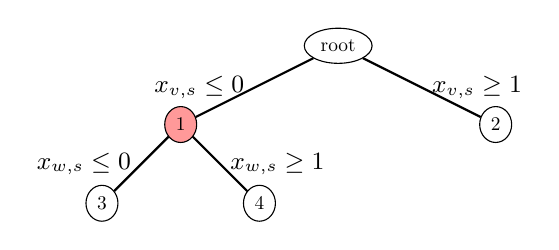
\begin{tikzpicture}
\usetikzlibrary{arrows}
\usetikzlibrary{shapes}
\tikzstyle{every node}=[draw, ellipse, minimum size=10pt,align=center,scale=0.7]
\node at ( 0, 0)(0) {root};
\node[fill=red!40] at (-2,-1)(1) {1};
\node at ( 2,-1)(2) {2};
\node at (-3,-2)(3) {3};
\node at (-1,-2)(4) {4};
\path[every node/.style={font=\sffamily\small},thick]
  (0) edge [] node [left] {$ x_{v,s} \leq 0$} (1)
  (0) edge [] node [right] {$ x_{v,s} \geq 1$} (2)
  (1) edge [] node [left] {$ x_{w,s} \leq 0$} (3)
  (1) edge [] node [right] {$ x_{w,s} \geq 1$} (4);
\end{tikzpicture}
\end{figure}
\end{frame}
\begin{frame}
\frametitle{Branch \& Price Algorithm}
\begin{figure}[h]
  \centering
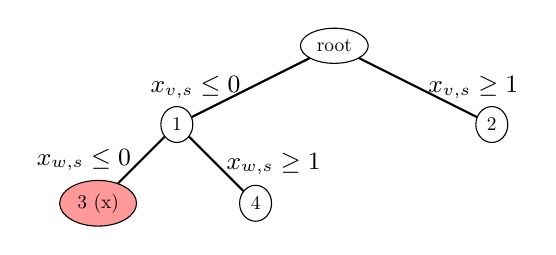
\begin{tikzpicture}
\usetikzlibrary{arrows}
\usetikzlibrary{shapes}
\tikzstyle{every node}=[draw, ellipse, minimum size=10pt,align=center,scale=0.7]
\node at ( 0, 0)(0) {root};
\node at (-2,-1)(1) {1};
\node at ( 2,-1)(2) {2};
\node[fill=red!40] at (-3,-2)(3) {3 (x)};
\node at (-1,-2)(4) {4};
\path[every node/.style={font=\sffamily\small},thick]
  (0) edge [] node [left] {$ x_{v,s} \leq 0$} (1)
  (0) edge [] node [right] {$ x_{v,s} \geq 1$} (2)
  (1) edge [] node [left] {$ x_{w,s} \leq 0$} (3)
  (1) edge [] node [right] {$ x_{w,s} \geq 1$} (4);
\end{tikzpicture}
\end{figure}
\end{frame}
\begin{frame}
\frametitle{Branch \& Price Algorithm}
\begin{figure}[h]
  \centering
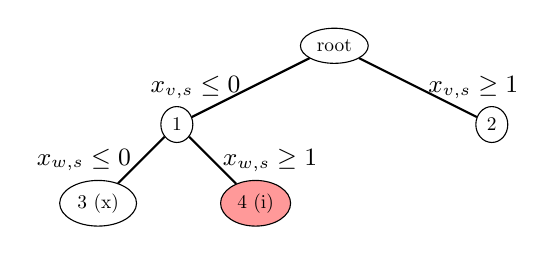
\begin{tikzpicture}
\usetikzlibrary{arrows}
\usetikzlibrary{shapes}
\tikzstyle{every node}=[draw, ellipse, minimum size=10pt,align=center,scale=0.7]
\node at ( 0, 0)(0) {root};
\node at (-2,-1)(1) {1};
\node at ( 2,-1)(2) {2};
\node at (-3,-2)(3) {3 (x)};
\node[fill=red!40] at (-1,-2)(4) {4 (i)};
\path[every node/.style={font=\sffamily\small},thick]
  (0) edge [] node [left] {$ x_{v,s} \leq 0$} (1)
  (0) edge [] node [right] {$ x_{v,s} \geq 1$} (2)
  (1) edge [] node [left] {$ x_{w,s} \leq 0$} (3)
  (1) edge [] node [right] {$ x_{w,s} \geq 1$} (4);
\end{tikzpicture}
\end{figure}
\end{frame}
\begin{frame}
\frametitle{Branch \& Price Algorithm}
\begin{figure}[h]
  \centering
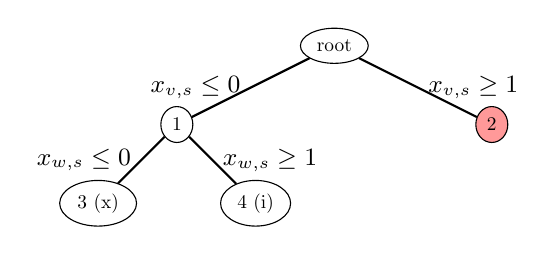
\begin{tikzpicture}
\usetikzlibrary{arrows}
\usetikzlibrary{shapes}
\tikzstyle{every node}=[draw, ellipse, minimum size=10pt,align=center,scale=0.7]
\node at ( 0, 0)(0) {root};
\node at (-2,-1)(1) {1};
\node[fill=red!40] at ( 2,-1)(2) {2};
\node at (-3,-2)(3) {3 (x)};
\node at (-1,-2)(4) {4 (i)};
\path[every node/.style={font=\sffamily\small},thick]
  (0) edge [] node [left] {$ x_{v,s} \leq 0$} (1)
  (0) edge [] node [right] {$ x_{v,s} \geq 1$} (2)
  (1) edge [] node [left] {$ x_{w,s} \leq 0$} (3)
  (1) edge [] node [right] {$ x_{w,s} \geq 1$} (4);
\end{tikzpicture}
\end{figure}
\end{frame}
%---------------------------
\begin{frame}
  \frametitle{B\&P details}
\begin{itemize}
  \item Variable selection
  \item Branching
	\item Node selection
  \item Heuristic at each node
\end{itemize}
\end{frame}
%---------------------------
\begin{frame}
  \frametitle{Variable Selection}
  Which variable is selected to be branched?
\begin{itemize}
  \item $x_{v,s}$ closest to $0.5$
  \item $z_{p}$ in order of origin node label, paths with the same origin are verified in order they were generated
\end{itemize}
\end{frame}
%---------------------------
\begin{frame}
  \frametitle{Branching}
  Node mapping variables
  \begin{itemize}
    \item Variable branching
    \begin{itemize}
      \item $x_{v,s} \leq 0$
      \item $x_{v,s} \geq 1$
    \end{itemize}
    \item Generalized Upper Bound (GUB)
    \begin{itemize}
      \item $\sum\limits_{s < |V^S| / 2} x_{v,s} \leq 0$
      \item $\sum\limits_{s > |V^S| / 2} x_{v,s} \leq 0$
    \end{itemize}
  \end{itemize}
  Link mapping variables
  \begin{itemize}
    \item Select two non-integral variables $z_{p}$ and $z_{p'}$
    \item Select physical edges $e \in p, e \notin p'$ and $f \in p', f \notin p$
    \begin{itemize}
      \item $\sum\limits_{p \in P^k} \delta_{e,p} z_p \leq 0$
      \item $\sum\limits_{p \in P^k} \delta_{f,p} z_p \leq 0$
    \end{itemize}
  \end{itemize}
\end{frame}
%---------------------------
\begin{frame}
  \frametitle{Node Selection}
\begin{itemize}
  \item DFS
  \item BFS
  \item Best Projection
\end{itemize}
\end{frame}
%---------------------------
\begin{frame}
  \frametitle{Heuristic Algorithm}
\begin{itemize}
  \item For each $v \in V^V$, round $x_{v,s}$
  \item For each $v \in E^V$, used BFS to find the path with fewest hops
\end{itemize}
\end{frame}
%---------------------------
\section{Experimental Results}

\begin{frame}
\frametitle{Experiments}
Experiments are divided in three steps
\begin{itemize}
  \item Parameter testing
  \item Branch \& Price Evaluation
  \item Amount of time spent by each component
\end{itemize}
\end{frame}
%---------------------------
\begin{frame}
\frametitle{Experimental Approach}
\begin{itemize}
  \item All tests were performed on processor Intel Core i7 930 with 12~Gb of memory. 
  \item The commercial solver CPLEX 12.5 was used to solve the relaxed and integer models. 
  \item All instances were generated using the GTI-ITM tool
  \item 3726 instances of more than 90 sizes
  \item Virtual Network Demand
    \begin{itemize}
      \item low demand 
      \item high demand
    \end{itemize}
  \item Topologies
    \begin{itemize}
      \item Sparse Random
      \item Dense Random
      \item Hierarchical
      \item Transit-stub
    \end{itemize}
\end{itemize}
\end{frame}
%---------------------------
\begin{frame}
  \frametitle{Parameter Testing}
  \begin{table}[h]
  \tiny
  \begin{center}
    \caption{Node Selection Results}\label{tab:nodesel}
  \begin{tabular} {l l | r r | r r | r r | r r }
  \hline
                  &                &  \multicolumn{2}{c|}{DFS}  & \multicolumn{2}{c|}{BFS}   & \multicolumn{2}{c|}{BPJ} & \multicolumn{2}{c}{Wilcox Signed-rank}  \\
    set           & \#inst           &  \#opt       & time(s)        & \#opt   & time(s)          & \#opt           & time(s)     & DFS $\sim$ BFS   & BPJ $\sim$ BFS  \\
   \hline 
   RS   & 108            & 76         & 1086.20    & 85        & 851.90       & 83            & 863.66   & < $10^{-3}$         & 0.991          \\
   RD   & 108            & 78         & 961.50     & 88        & 792.10       & 87            & 691.44   & < $10^{-3}$         & 0.994          \\ 
   H    & 108            & 62         & 1503.62    & 64        & 1375.61      & 59            & 1542.29  & < $10^{-3}$         & 0.035          \\
   Ts   & 90             & 59         & 1393.76    & 66        & 1138.92      & 62            & 1294.34  & < $10^{-3}$         & 0.003          \\
  \hline
  \end{tabular}
  \end{center}
  \end{table}
\begin{itemize}
  \item GUB x variable branching: variable branching is better with a confidence interval of 95\%
  \item Use of constructive heuristic: no statistical conclusion, but average is 6 seconds better
\end{itemize}
\end{frame}
%---------------------------
\begin{frame}
  \frametitle{Branch \& Price}
  \begin{figure}
          \begin{subfigure}[b]{0.47\textwidth}
                  \includegraphics[width=\textwidth]{graphs/time_fdensevir4}
                  \caption{Time}
          \end{subfigure}
          ~
          \begin{subfigure}[b]{0.47\textwidth}
                  \includegraphics[width=\textwidth]{graphs/cost_fdensevir4}
                  \caption{Cost}
          \end{subfigure}
  \end{figure}
  Dense Random - high demand
\end{frame}
%---------------------------
\begin{frame}
  \frametitle{Branch \& Price}
  \begin{figure}
          \begin{subfigure}[b]{0.47\textwidth}
                  \includegraphics[width=\textwidth]{graphs/fint_fdensevir4}
                  \caption{First Integer Solution}
          \end{subfigure}
          ~
          \begin{subfigure}[b]{0.47\textwidth}
                  \includegraphics[width=\textwidth]{graphs/opt_fdensevir4}
                  \caption{\# Proved Optimal}
          \end{subfigure}
  \end{figure}
  Dense Random - high demand
\end{frame}
%---------------------------
\begin{frame}
  \frametitle{Amount of time spent by each component}

\begin{table}[h]
\begin{center}
\tiny
\begin{tabular} { l | r r r r | r r r r }
\hline
% low demand / high demand
             &  \multicolumn{4}{c|}{Low Demand}                            & \multicolumn{4}{c}{High Demand} \\
Set          &  master(\%) &  add(\%)      &   pric(\%)            &  aux(\%)     & master(\%) &            add(\%)       &             pric(\%)  &  aux(\%) \\
\hline
Sparse       &  6.07   &            0.32             &               49.22  &  12.14  &  10.41  &            0.04             &               42.76  &  13.23  \\
Dense        &  3.55   &            0.21             &               52.61  &  13.62  &  7.83   &            0.07             &               48.51  &  11.14  \\
Hierarchical &  20.36  &            0.00             &               33.32  &  25.35  &  17.12  &            0.01             &               39.24  &  23.17  \\
Transit-stub &  13.66  &            0.01             &               35.93  &  29.02  &  14.19  &            0.00             &               38.46  &  25.97  \\
\hline
\end{tabular} 
\end{center}
\end{table}
\end{frame}
%---------------------------
\section{Concluding Remarks}
\begin{frame}
\frametitle{Concluding Remarks}
Contribution
\begin{itemize}
  \item Characterization of VNEP complexity
	\item New Branch \& Price for VNEP with single-paths
  \item New algorithm for pricing problem
  \item Proposed algorithm is able to solve larger instances in less time than CPLEX implementation
  \item Proposed algorithm can be used to solve small instances in practice and be used to evaluate heuristic algorithms
\end{itemize}
\end{frame}
%---------------------------
\begin{frame}
\frametitle{Concluding Remarks}
Future research directions
\begin{itemize}
  \item Improvement of Column Generation
  \begin{itemize}
    \item Generation of a single column at each iteration
    \item Use of a dynamic algorithm
  \end{itemize}
  \item Extension of algorithm to a Branch \& Price \& Cut by using cover inequalities
  \item Adaptation of the algorithm to deal with multiple requests simultaneously
\end{itemize}
\end{frame}
%---------------------------
\begin{frame}
\frametitle{}
\begin{center} 
  { \huge Thank you }
  
  \bigskip
  Leonardo Moura \\
  \textit{lfsmoura@inf.ufrgs.br}
  \begin{figure}
      \centering
      \includegraphics[scale=0.4]{inf.png}
  \end{figure}
\end{center}
\end{frame}
%----------------------------------------------------
%  E X T R A
%----------------------------------------------------
\begin{frame}
\frametitle{Improving Lower Bounds}
Dantzig-Wolfe Decomposition provides models with better lower bounds
\pause
\begin{align}
  & \sum\limits_{(v,w) \in E^{V}} B_{vw}  y_{vwst} \leq B_{st}                 & \forall (s,t) \in E^{S} \nonumber \\
  & \sum\limits_{t \in V^{S}} ( y_{vwst} - y_{vwts}) = x_{vs} - x_{ws} & \forall (v,w) \in E^{V} \nonumber  
\end{align}

\begin{equation}
A = \left[  \begin{array}{cccc}
            A_{1} & A_{2} & \ldots & A_{p} \\
            B_{1} &       &        &       \\
                  & B_{2} &        &       \\
                  &       & \ddots &       \\
                  &       &        & B_{p} \\
            \end{array} \right] \nonumber
\end{equation}
\end{frame}
\begin{frame}
  \frametitle{Dantzig-Wolfe decomposition}
A nonempty and bounded convex polyhedron can be represented by a convex combination of its extreme points (LASDON, 1970).

\begin{align}
  y_{k} = & \sum\limits_{p \in P^{k}} \delta_{p} z_{p} \nonumber & \\
        %& x_{v,s} = \sum\limits_{(v,w) \in E^V} \sum\limits_{p \in P^{(v,w)}} \delta_{v,s,p} z_{p}
          & \sum\limits_{p \in P^k} z_{p} = 1 & \forall k \in E^V \nonumber \\
          & z_{p} \in \{0,1\}                       & \forall k \in E^V, p \in P^k \nonumber
\end{align}
\end{frame}
\begin{frame}
  \frametitle{Best Projection}
  \begin{equation}
    \phi(i) = z_{i}^* + (\frac{UB - z_{root}^*}{s_{root}}) s_{i}   \nonumber
  \end{equation}

  \begin{equation}
    s_{i} = \sum \min \{ x_{j} - \lfloor x_{j} \rfloor, \lceil x_{j} \rceil - x_{j} \} \nonumber
  \end{equation}

  ex: $\min\{2.7 - 2, 3 - 2.7\} = 0.3$

\end{frame}


\begin{comment}
\begin{frame}[allowframebreaks]
\bibliographystyle{apalike}
\bibliography{VNE}
\end{frame}
\end{comment}


\end{document}

%---------------------------
\begin{frame}
\frametitle{teste}

\end{frame}

